% Swiss edition plates: painted Nano Banana Pro renders in a Swiss-modern
% register (flat colour blocking, hard edges, no gradients, no outlines, no
% type), replacing the earlier TikZ-drawn plates. Art direction is
% docs/harbor-research/exposition/SWISS-BRIEF.md; the thirteen renders, their
% prompts, and their post-processing are recorded in
% book/plates/swiss/PROVENANCE.json. The cover render
% was generated first and then attached as the STYLE TEMPLATE reference to
% every other plate so the thirteen hold together as one set.
%
% \pdswisscoverart draws nothing itself: it makes the cover render the page's
% full-bleed background, leaving the reserved top-left paper for the type the
% TeX sets over it (the cover's title sits at fixed overlay coordinates, so a
% full-bleed image behind it is always safe). \pdswisspartplate{<numeral>}{<width>}
% and \pdswissplate{<prefix>}{<width>} both stay real inline content
% placed after the flowing title/blurb/question text, each at the given
% width and the old TikZ drawing's own aspect (part: 3:2, 24x16 units;
% chapter: 2:1, 24x12 units). There is no drawn fallback: a missing render
% stops the build with a \PackageError naming the missing path.
\makeatletter
\newcommand{\pdswisscoverart}{%
  \IfFileExists{plates/swiss/cover.jpg}{%
    \AddToShipoutPictureBG*{\AtPageLowerLeft{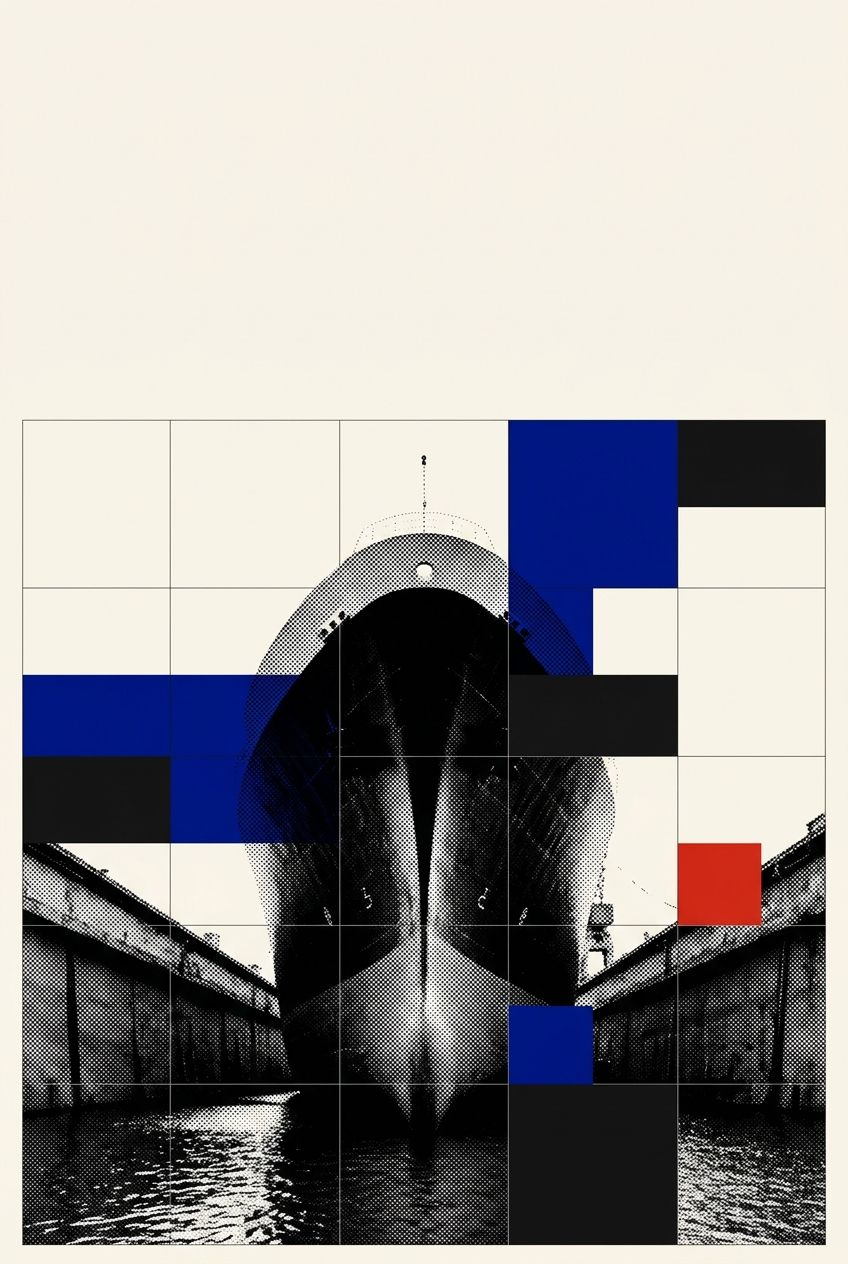
\includegraphics[width=\paperwidth,height=\paperheight]{plates/swiss/cover.jpg}}}}{%
    \PackageError{pd-swiss-plates}{Missing plate render plates/swiss/cover.jpg}{Generate the Swiss cover render and place it at plates/swiss/cover.jpg before building.}}}
\newcommand{\pdswisspartplate}[2]{% #1 numeral I..IV, #2 width
  \IfFileExists{plates/swiss/part-#1.jpg}{%
    \includegraphics[width=#2]{plates/swiss/part-#1.jpg}}{%
    \PackageError{pd-swiss-plates}{Missing plate render plates/swiss/part-#1.jpg}{Generate the Swiss part plate render and place it at plates/swiss/part-#1.jpg before building.}}}
\newcommand{\pdswissplate}[2]{% #1 chapter prefix, #2 width
  \IfFileExists{plates/swiss/chapter-#1.jpg}{%
    \includegraphics[width=#2]{plates/swiss/chapter-#1.jpg}%
  }{%
    \PackageError{pd-swiss-plates}{Missing plate render plates/swiss/chapter-#1.jpg}{Generate the Swiss chapter plate render and place it at plates/swiss/chapter-#1.jpg before building.}%
  }%
}
\newcommand{\pdswissfigplate}[2]{% #1 figure name, #2 width
  \IfFileExists{plates/swiss/#1.jpg}{%
    \includegraphics[width=#2]{plates/swiss/#1.jpg}%
  }{%
    \PackageError{pd-swiss-plates}{Missing figure plate render plates/swiss/#1.jpg}{Generate the Swiss figure plate render and place it at plates/swiss/#1.jpg before building.}%
  }%
}
\providecolor{pdswissred}{HTML}{DA291C}
\providecolor{pdcobalt}{HTML}{001489}
\providecolor{hhink}{HTML}{1B1712}
\providecolor{hhgray}{HTML}{5C5650}

% Canonical Landmark titles and pull-quotes
\expandafter\def\csname pdlandmarktitle@01\endcsname{The Substrate Bedrock \& The Kernel Gap}
\expandafter\def\csname pdlandmarkconcept@01\endcsname{Substrate Bedrock \& The Operating Kernel Gap}
\expandafter\def\csname pdlandmarkquestion@01\endcsname{Which effects require mediation, and which records must survive a failure?}
\expandafter\def\csname pdlandmarkquote@01\endcsname{A proposed action is not evidence that it occurred. A state-dependent admission rule needs adequate evidence of the state on which it depends. When recovery depends on a past event, an adequate record must survive the failure being considered.}

\expandafter\def\csname pdlandmarktitle@02\endcsname{Agentic Continuity \& The Overlapping Strand}
\expandafter\def\csname pdlandmarkconcept@02\endcsname{Substrate Continuity \& Overlapping Strands}
\expandafter\def\csname pdlandmarkquestion@02\endcsname{What makes an obligation survive a change of worker?}
\expandafter\def\csname pdlandmarkquote@02\endcsname{Continuity belongs to a maintained record of authority, obligations and evidence. Processes and models may change while that record persists. A succession rule must identify who inherits each obligation; similarity of behavior alone does not establish accountable identity.}

\expandafter\def\csname pdlandmarktitle@03\endcsname{The Engine Swap}
\expandafter\def\csname pdlandmarkconcept@03\endcsname{The Engine Swap \& Model Portability}
\expandafter\def\csname pdlandmarkquestion@03\endcsname{What must be checked before a replacement model continues the work?}
\expandafter\def\csname pdlandmarkquote@03\endcsname{A model can be replaced without discarding the work record. Safe continuation still requires compatible tools, retained obligations and checks on the replacement worker. Preserving a contract does not establish that the new model can fulfill it.}

\expandafter\def\csname pdlandmarktitle@04\endcsname{The Front-Loaded Probation Cliff}
\expandafter\def\csname pdlandmarkconcept@04\endcsname{The Front-Loaded Probation Cliff}
\expandafter\def\csname pdlandmarkquestion@04\endcsname{What does probation establish, and what risk remains?}
\expandafter\def\csname pdlandmarkquote@04\endcsname{Probation limits exposure while evidence accumulates. Admission depends on an explicit rule, the quality of the evidence and the cost of a mistake. A successful history can justify a bounded grant; it cannot prove that future behavior will be harmless.}

\expandafter\def\csname pdlandmarktitle@05\endcsname{The Single-Writer Monotonic Horizon}
\expandafter\def\csname pdlandmarkconcept@05\endcsname{The Single-Writer Monotonic Horizon}
\expandafter\def\csname pdlandmarkquestion@05\endcsname{What does a local commit order settle, and what lies outside it?}
\expandafter\def\csname pdlandmarkquote@05\endcsname{Within its mediated domain, a serializing writer can give admitted transactions a common commit order. Durability depends on the storage and failure model. That local order does not by itself resolve disagreement between independent operators or prevent effects outside the writer.}

\expandafter\def\csname pdlandmarktitle@06\endcsname{The Attenuation Frontier \& Cryptographic Macaroons}
\expandafter\def\csname pdlandmarkconcept@06\endcsname{The Attenuation Frontier \& Macaroons}
\expandafter\def\csname pdlandmarkquestion@06\endcsname{When does delegation actually narrow authority?}
\expandafter\def\csname pdlandmarkquote@06\endcsname{An attenuated credential adds restrictions to an existing grant. Authority narrows only when the verifier checks the complete delegation chain and enforces every applicable restriction. Possessing a signed credential is not sufficient authorization for an arbitrary action.}

\expandafter\def\csname pdlandmarktitle@07\endcsname{Attestation Without Revelation (The Sealed Harbor)}
\expandafter\def\csname pdlandmarkconcept@07\endcsname{Attestation Without Revelation (Sealed Harbor)}
\expandafter\def\csname pdlandmarkquestion@07\endcsname{What does attestation establish about a private computation?}
\expandafter\def\csname pdlandmarkquote@07\endcsname{Attestation can identify a measured execution environment under a stated trust model. It does not alone prove that a program is correct or that its outputs reveal no private information. Those claims require separate specifications, enforcement and evidence.}

\expandafter\def\csname pdlandmarktitle@08\endcsname{Read-Poverty \& The Legible Swarm}
\expandafter\def\csname pdlandmarkconcept@08\endcsname{Read-Poverty \& Stigmergic Signaling}
\expandafter\def\csname pdlandmarkquestion@08\endcsname{Which evidence is worth an operator's limited attention?}
\expandafter\def\csname pdlandmarkquote@08\endcsname{An operator has a finite inspection budget. Structured summaries and accessible evidence can reduce the cost of a particular decision. Their value depends on what they preserve and what errors they hide; a shorter message is not automatically a better account.}

\expandafter\def\csname pdlandmarktitle@09\endcsname{Skills as Capital vs.\ Token Labor}
\expandafter\def\csname pdlandmarkconcept@09\endcsname{Skills as Capital vs. Perishable Token Labor}
\expandafter\def\csname pdlandmarkquestion@09\endcsname{When does a reusable tool repay its construction cost?}
\expandafter\def\csname pdlandmarkquote@09\endcsname{A reusable tool trades an initial construction and verification cost for repeated execution. It pays off only when sufficient valid uses recover that cost, including maintenance. Deliberation remains necessary where inputs, requirements or the tool itself are uncertain.}

\expandafter\def\csname pdlandmarktitle@10\endcsname{Bonds, Evidence \& Settlement}
\expandafter\def\csname pdlandmarkconcept@10\endcsname{Bonds, Evidence \& Settlement}
\expandafter\def\csname pdlandmarkquestion@10\endcsname{When can a bond deter a violation that evidence can establish?}
\expandafter\def\csname pdlandmarkquote@10\endcsname{A bond changes incentives only when a violation can be established and the sanction collected. Coverage, detection and deterrence are separate calculations. Settlement must follow the agreed evidence and dispute rules; collateral does not make every harmful action observable.}

\expandafter\def\csname pdlandmarktitle@11\endcsname{Cycle Consistency \& Its Limits}
\expandafter\def\csname pdlandmarkconcept@11\endcsname{Sheaf Laplacians \& Cycle Holonomy}
\expandafter\def\csname pdlandmarkquestion@11\endcsname{Which inconsistencies can cycle checks expose, and which can they miss?}
\expandafter\def\csname pdlandmarkquote@11\endcsname{Cycle checks compare recorded claims under specified observation and restriction maps. A nonzero residual witnesses inconsistency in those records; it does not identify a liar or establish malicious intent. Zero residual also leaves the observation model's blind spots unresolved.}

\expandafter\def\csname pdlandmarktitle@12\endcsname{The Zombie Reclaim \& Salvage Graveyard}
\expandafter\def\csname pdlandmarkconcept@12\endcsname{Zombie Salvage \& Dead-Man Leases}
\expandafter\def\csname pdlandmarkquestion@12\endcsname{How can work be reassigned without admitting a stale worker?}
\expandafter\def\csname pdlandmarkquote@12\endcsname{A missing heartbeat is evidence of silence, not proof of death. Reassignment requires an expiry rule, retained work state and fencing that rejects a stale holder's writes to the reassigned resource. Recovery must also account for effects whose completion was never recorded.}

% Single-digit alias fallbacks
\expandafter\def\csname pdlandmarktitle@1\endcsname{\csname pdlandmarktitle@01\endcsname}
\expandafter\def\csname pdlandmarkconcept@1\endcsname{\csname pdlandmarkconcept@01\endcsname}
\expandafter\def\csname pdlandmarkquestion@1\endcsname{\csname pdlandmarkquestion@01\endcsname}
\expandafter\def\csname pdlandmarkquote@1\endcsname{\csname pdlandmarkquote@01\endcsname}

\expandafter\def\csname pdlandmarktitle@2\endcsname{\csname pdlandmarktitle@02\endcsname}
\expandafter\def\csname pdlandmarkconcept@2\endcsname{\csname pdlandmarkconcept@02\endcsname}
\expandafter\def\csname pdlandmarkquestion@2\endcsname{\csname pdlandmarkquestion@02\endcsname}
\expandafter\def\csname pdlandmarkquote@2\endcsname{\csname pdlandmarkquote@02\endcsname}

\expandafter\def\csname pdlandmarktitle@3\endcsname{\csname pdlandmarktitle@03\endcsname}
\expandafter\def\csname pdlandmarkconcept@3\endcsname{\csname pdlandmarkconcept@03\endcsname}
\expandafter\def\csname pdlandmarkquestion@3\endcsname{\csname pdlandmarkquestion@03\endcsname}
\expandafter\def\csname pdlandmarkquote@3\endcsname{\csname pdlandmarkquote@03\endcsname}

\expandafter\def\csname pdlandmarktitle@4\endcsname{\csname pdlandmarktitle@04\endcsname}
\expandafter\def\csname pdlandmarkconcept@4\endcsname{\csname pdlandmarkconcept@04\endcsname}
\expandafter\def\csname pdlandmarkquestion@4\endcsname{\csname pdlandmarkquestion@04\endcsname}
\expandafter\def\csname pdlandmarkquote@4\endcsname{\csname pdlandmarkquote@04\endcsname}

\expandafter\def\csname pdlandmarktitle@5\endcsname{\csname pdlandmarktitle@05\endcsname}
\expandafter\def\csname pdlandmarkconcept@5\endcsname{\csname pdlandmarkconcept@05\endcsname}
\expandafter\def\csname pdlandmarkquestion@5\endcsname{\csname pdlandmarkquestion@05\endcsname}
\expandafter\def\csname pdlandmarkquote@5\endcsname{\csname pdlandmarkquote@05\endcsname}

\expandafter\def\csname pdlandmarktitle@6\endcsname{\csname pdlandmarktitle@06\endcsname}
\expandafter\def\csname pdlandmarkconcept@6\endcsname{\csname pdlandmarkconcept@06\endcsname}
\expandafter\def\csname pdlandmarkquestion@6\endcsname{\csname pdlandmarkquestion@06\endcsname}
\expandafter\def\csname pdlandmarkquote@6\endcsname{\csname pdlandmarkquote@06\endcsname}

\expandafter\def\csname pdlandmarktitle@7\endcsname{\csname pdlandmarktitle@07\endcsname}
\expandafter\def\csname pdlandmarkconcept@7\endcsname{\csname pdlandmarkconcept@07\endcsname}
\expandafter\def\csname pdlandmarkquestion@7\endcsname{\csname pdlandmarkquestion@07\endcsname}
\expandafter\def\csname pdlandmarkquote@7\endcsname{\csname pdlandmarkquote@07\endcsname}

\expandafter\def\csname pdlandmarktitle@8\endcsname{\csname pdlandmarktitle@08\endcsname}
\expandafter\def\csname pdlandmarkconcept@8\endcsname{\csname pdlandmarkconcept@08\endcsname}
\expandafter\def\csname pdlandmarkquestion@8\endcsname{\csname pdlandmarkquestion@08\endcsname}
\expandafter\def\csname pdlandmarkquote@8\endcsname{\csname pdlandmarkquote@08\endcsname}

\expandafter\def\csname pdlandmarktitle@9\endcsname{\csname pdlandmarktitle@09\endcsname}
\expandafter\def\csname pdlandmarkconcept@9\endcsname{\csname pdlandmarkconcept@09\endcsname}
\expandafter\def\csname pdlandmarkquestion@9\endcsname{\csname pdlandmarkquestion@09\endcsname}
\expandafter\def\csname pdlandmarkquote@9\endcsname{\csname pdlandmarkquote@09\endcsname}

\newcommand{\pdswisslandmarkplate}[2]{% #1 landmark ID (e.g. 01..12), #2 width
  \IfFileExists{plates/swiss/landmark-#1.jpg}{%
    \centering
    \includegraphics[width=#2]{plates/swiss/landmark-#1.jpg}%
    \par\vspace{10pt}%
    \begin{minipage}{\linewidth}%
      {\color{pdcobalt}\rule{\linewidth}{1.2pt}}\par\vspace{6pt}%
      \raggedright
      {\color{pdswissred}\rule{4.5pt}{4.5pt}}\enspace%
      {\pdgrotesk\bfseries\scshape\fontsize{9}{11}\selectfont\color{hhink}%
        Landmark #1\enspace\textperiodcentered\enspace\csname pdlandmarktitle@#1\endcsname}\par\vspace{4.5pt}%
      {\pdgrotesk\itshape\fontsize{9.5}{13.5}\selectfont\color{hhink}%
        \csname pdlandmarkquote@#1\endcsname\par}%
      \vspace{6pt}%
      {\color{hhgray!30}\rule{\linewidth}{0.4pt}}%
    \end{minipage}%
  }{%
    \PackageError{pd-swiss-plates}{Missing plate render plates/swiss/landmark-#1.jpg}{Generate the Swiss landmark plate render and place it at plates/swiss/landmark-#1.jpg before building.}}}
\makeatother
